\documentclass{article}
\usepackage[utf8]{inputenc}
\usepackage[left=35mm,top=26mm,right=26mm,bottom=15mm]{geometry}
\usepackage{amsmath}
\usepackage{bigints}
\usepackage{graphicx}

\title{\Huge AE 227 Assignment 6}
\author{\Huge Krishna Wadhwani - 160010031 }
\date{November 2017}

\begin{document}

\maketitle

\section{Question 1}

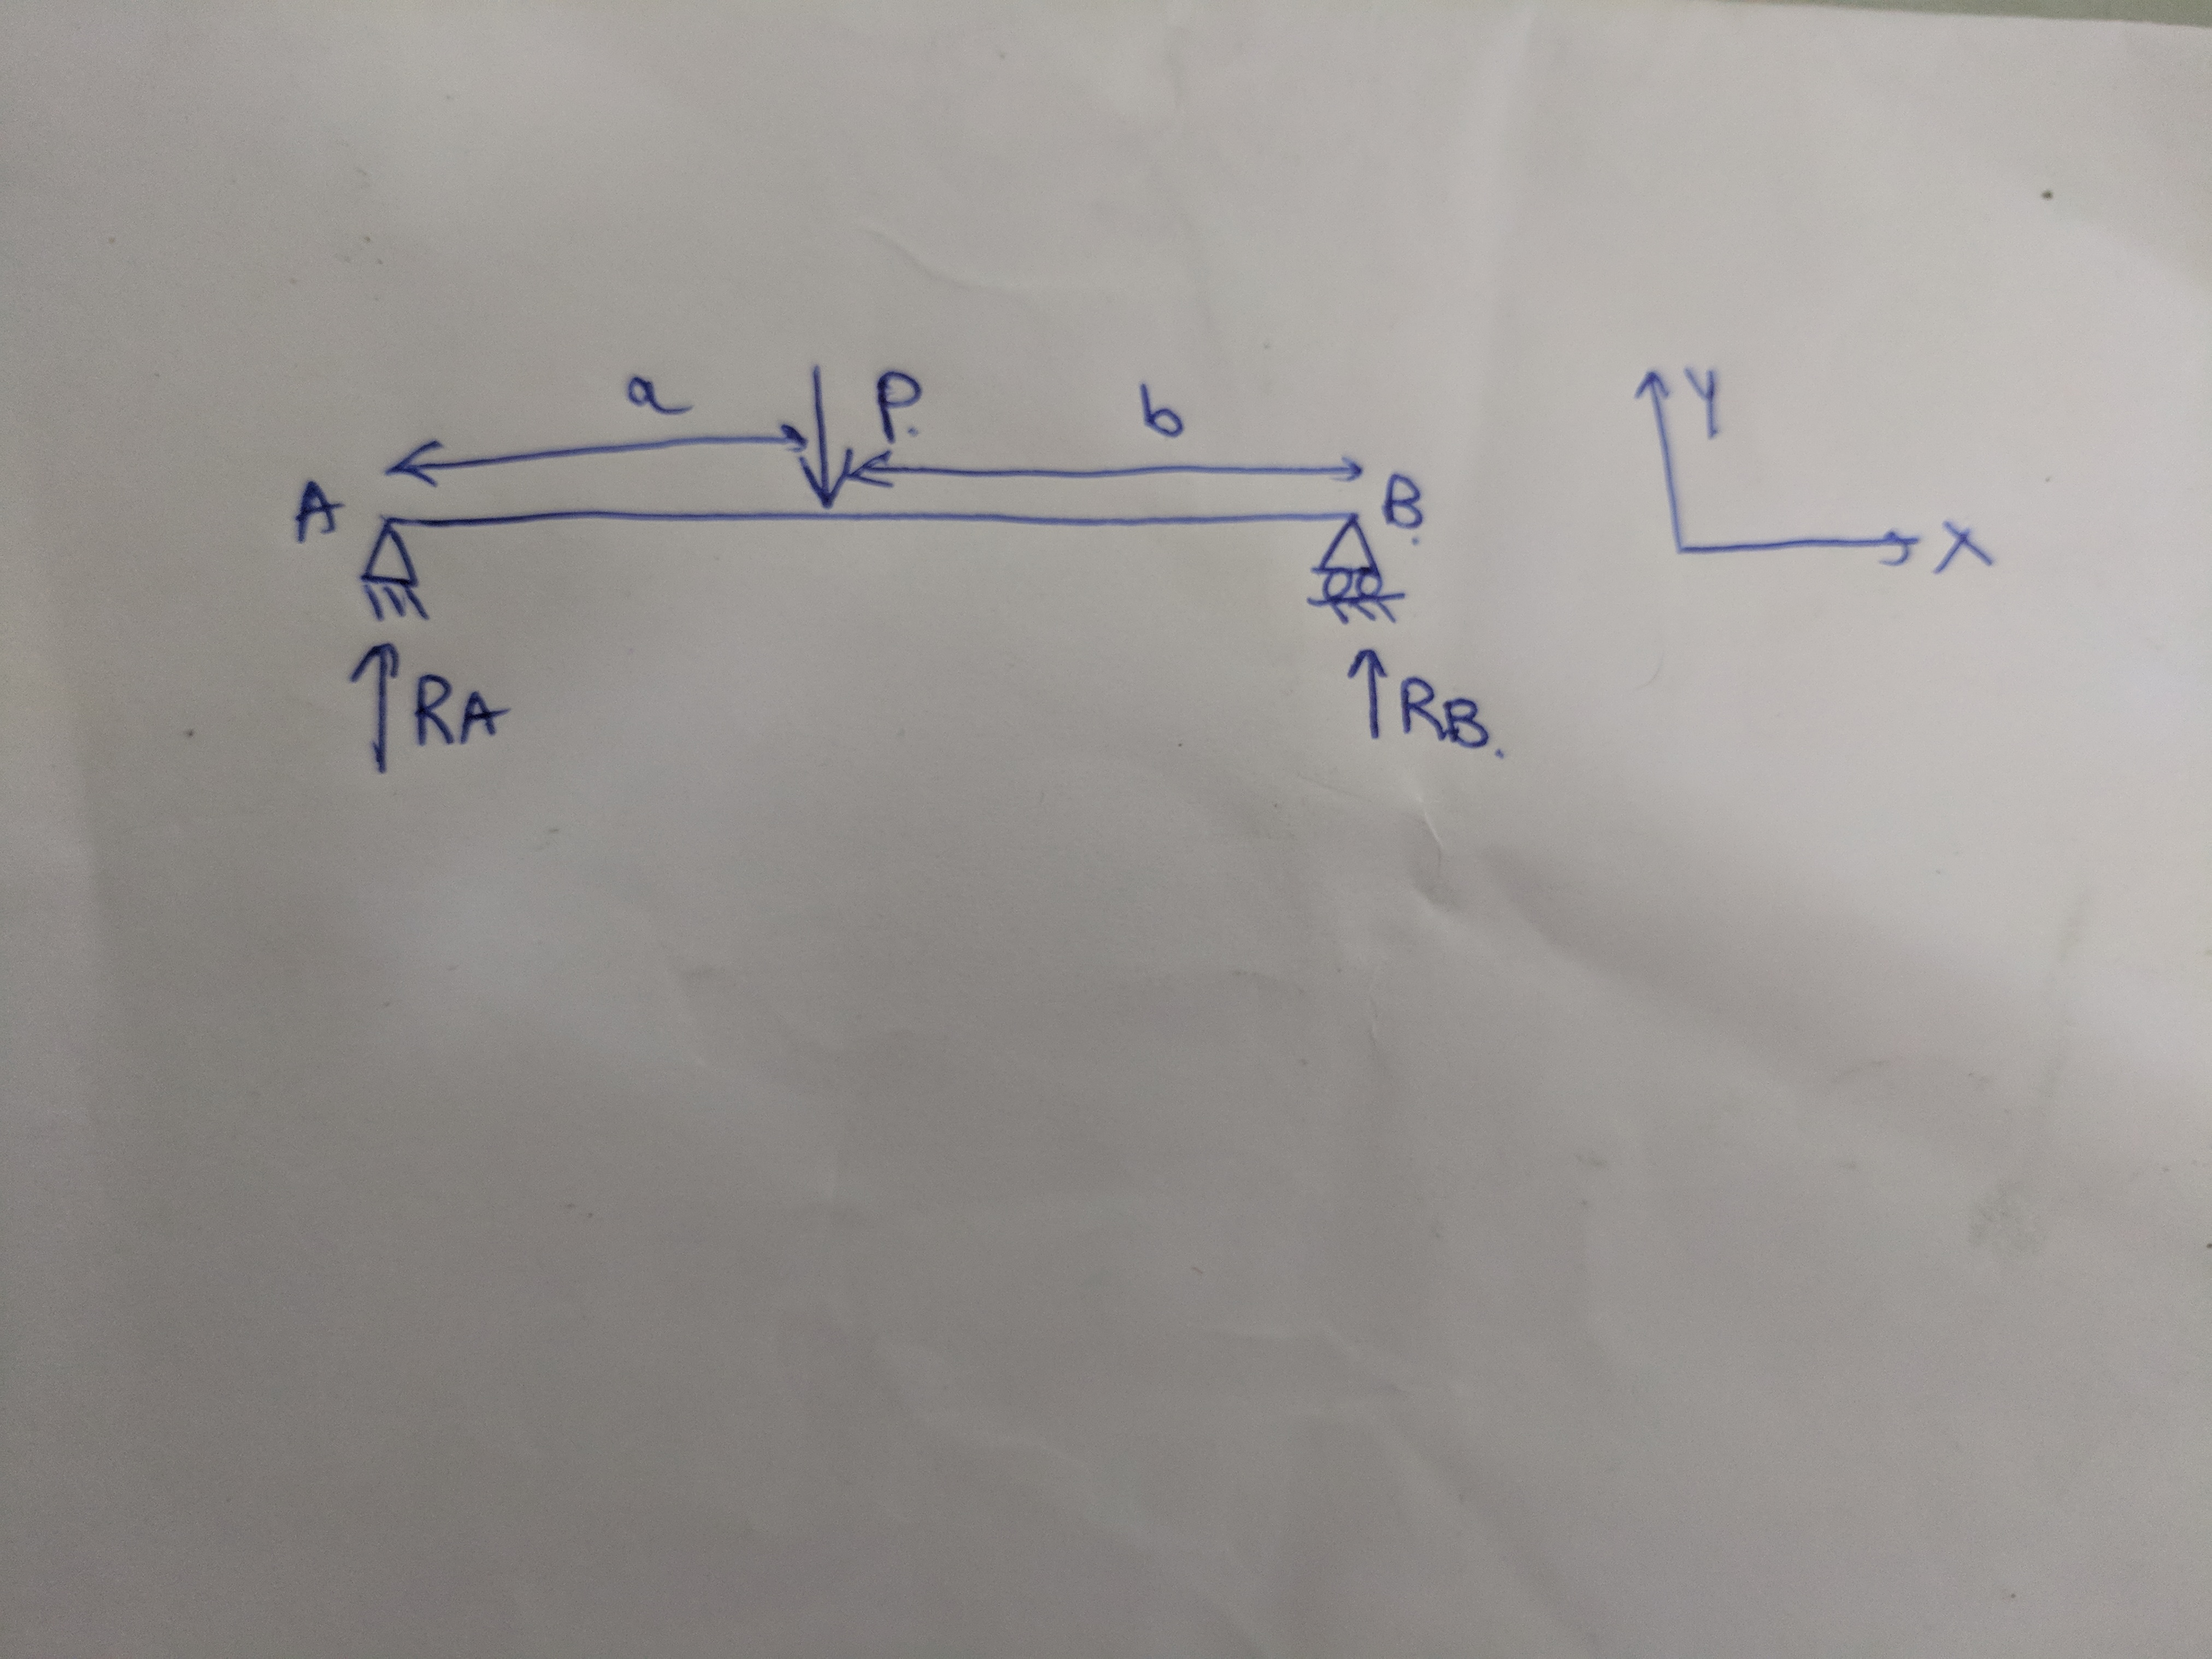
\includegraphics[scale=0.05]{Q1.jpg}

\noindent First we will solve the beam to determine reaction forces $R_A$ and $R_B$.\\

\noindent Applying force equilibrium along $y$: \\
$R_A+R_B-P=0 \ \ \hdots eq^n 1$\\

\noindent Applying moment equilibrium about point A:\\
$-Pa+R_B(a+b)=0$\\
$\implies R_B =\dfrac{Pa}{L}$\\

\noindent From $eq^n 1$: $R_A=\dfrac{Pb}{L}$\\

\noindent where $L=a+b$\\

\noindent We need to find deflection of the beam using energy method. 

\noindent $\dfrac{1}{2}P\gamma = U$\\
where $\gamma$ is deflection of the beam and $U=\bigint\limits_0^L\dfrac{M(x)^2}{2EI}dx$\\
Solving for U:\\
$U=\bigint\limits_0^a\dfrac{M(x)^2}{2EI}dx +\bigint\limits_a^L\dfrac{M(x)^2}{2EI}dx $\\

\noindent To further solve the equation, we need to obtain the expression of $M(x)$\\

\noindent For the region $0<x<a$:\\
Moment equilibrium about point X:\\
$M-R_Ax=0$\\
$\implies M=\dfrac{Pbx}{L}$\\

\noindent For the region $a<x<L$:\\
Moment equilibrium about point X:\\
$M-R_Ax+P(x-a)=0$\\
$\implies M=\dfrac{Pa(L-x)}{L}$\\

\noindent Now using $M(x)$ to obatin the expression for $U$:\\
$U=\bigint\limits_0^a\dfrac{\Big (\dfrac{Pbx}{L} \Big )^2}{2EI}dx +\bigint\limits_a^L\dfrac{\Big (\dfrac{Pa(L-x)}{L} \Big)^2}{2EI}dx $\\
$\implies U= \dfrac{P^2b^2a^3}{6EIL^2}+\dfrac{P^2a^2b^3}{6EIL^2}$\\

\noindent $\implies U= \dfrac{P^2b^2a^2(a+b)}{6EIL^2}$\\
$\implies U= \dfrac{P^2b^2a^2}{6EIL}$\\

\noindent As $\dfrac{1}{2}P\nu = U$\\
$\implies \nu=\dfrac{2U}{P}$\\
$\nu= \dfrac{Pb^2a^2}{3EIL} = \dfrac{Pb^2a^2}{3EI(a+b)}$\\

\noindent For Maximum sheer force, we need to consider sheer force along the beam (Let the cross-section of the beam be A): 

\noindent For the region $0<x<a$:\\
$S_1=R_A=\dfrac{Pb}{L}$\\
$\sigma_{xy1}=\dfrac{Pb}{AL}$

\noindent For the region $a<x<L$:\\
$S_2=R_A-P=-\dfrac{Pa}{L}$\\
$\sigma_{xy2}=-\dfrac{Pa}{AL}$\\

\noindent where $\sigma_{xy}$ denoted sheer stress.\\

\noindent So maximum sheer stress $\sigma_{xy_{max}}= max\bigg(\dfrac{Pb}{AL}, \dfrac{Pa}{AL}\bigg)$ (Considering magnitude). \\
Let $b>a$. So $\sigma_{xy_{max}}=\dfrac{Pb}{AL}$

\bigbreak

\section{Question 2}

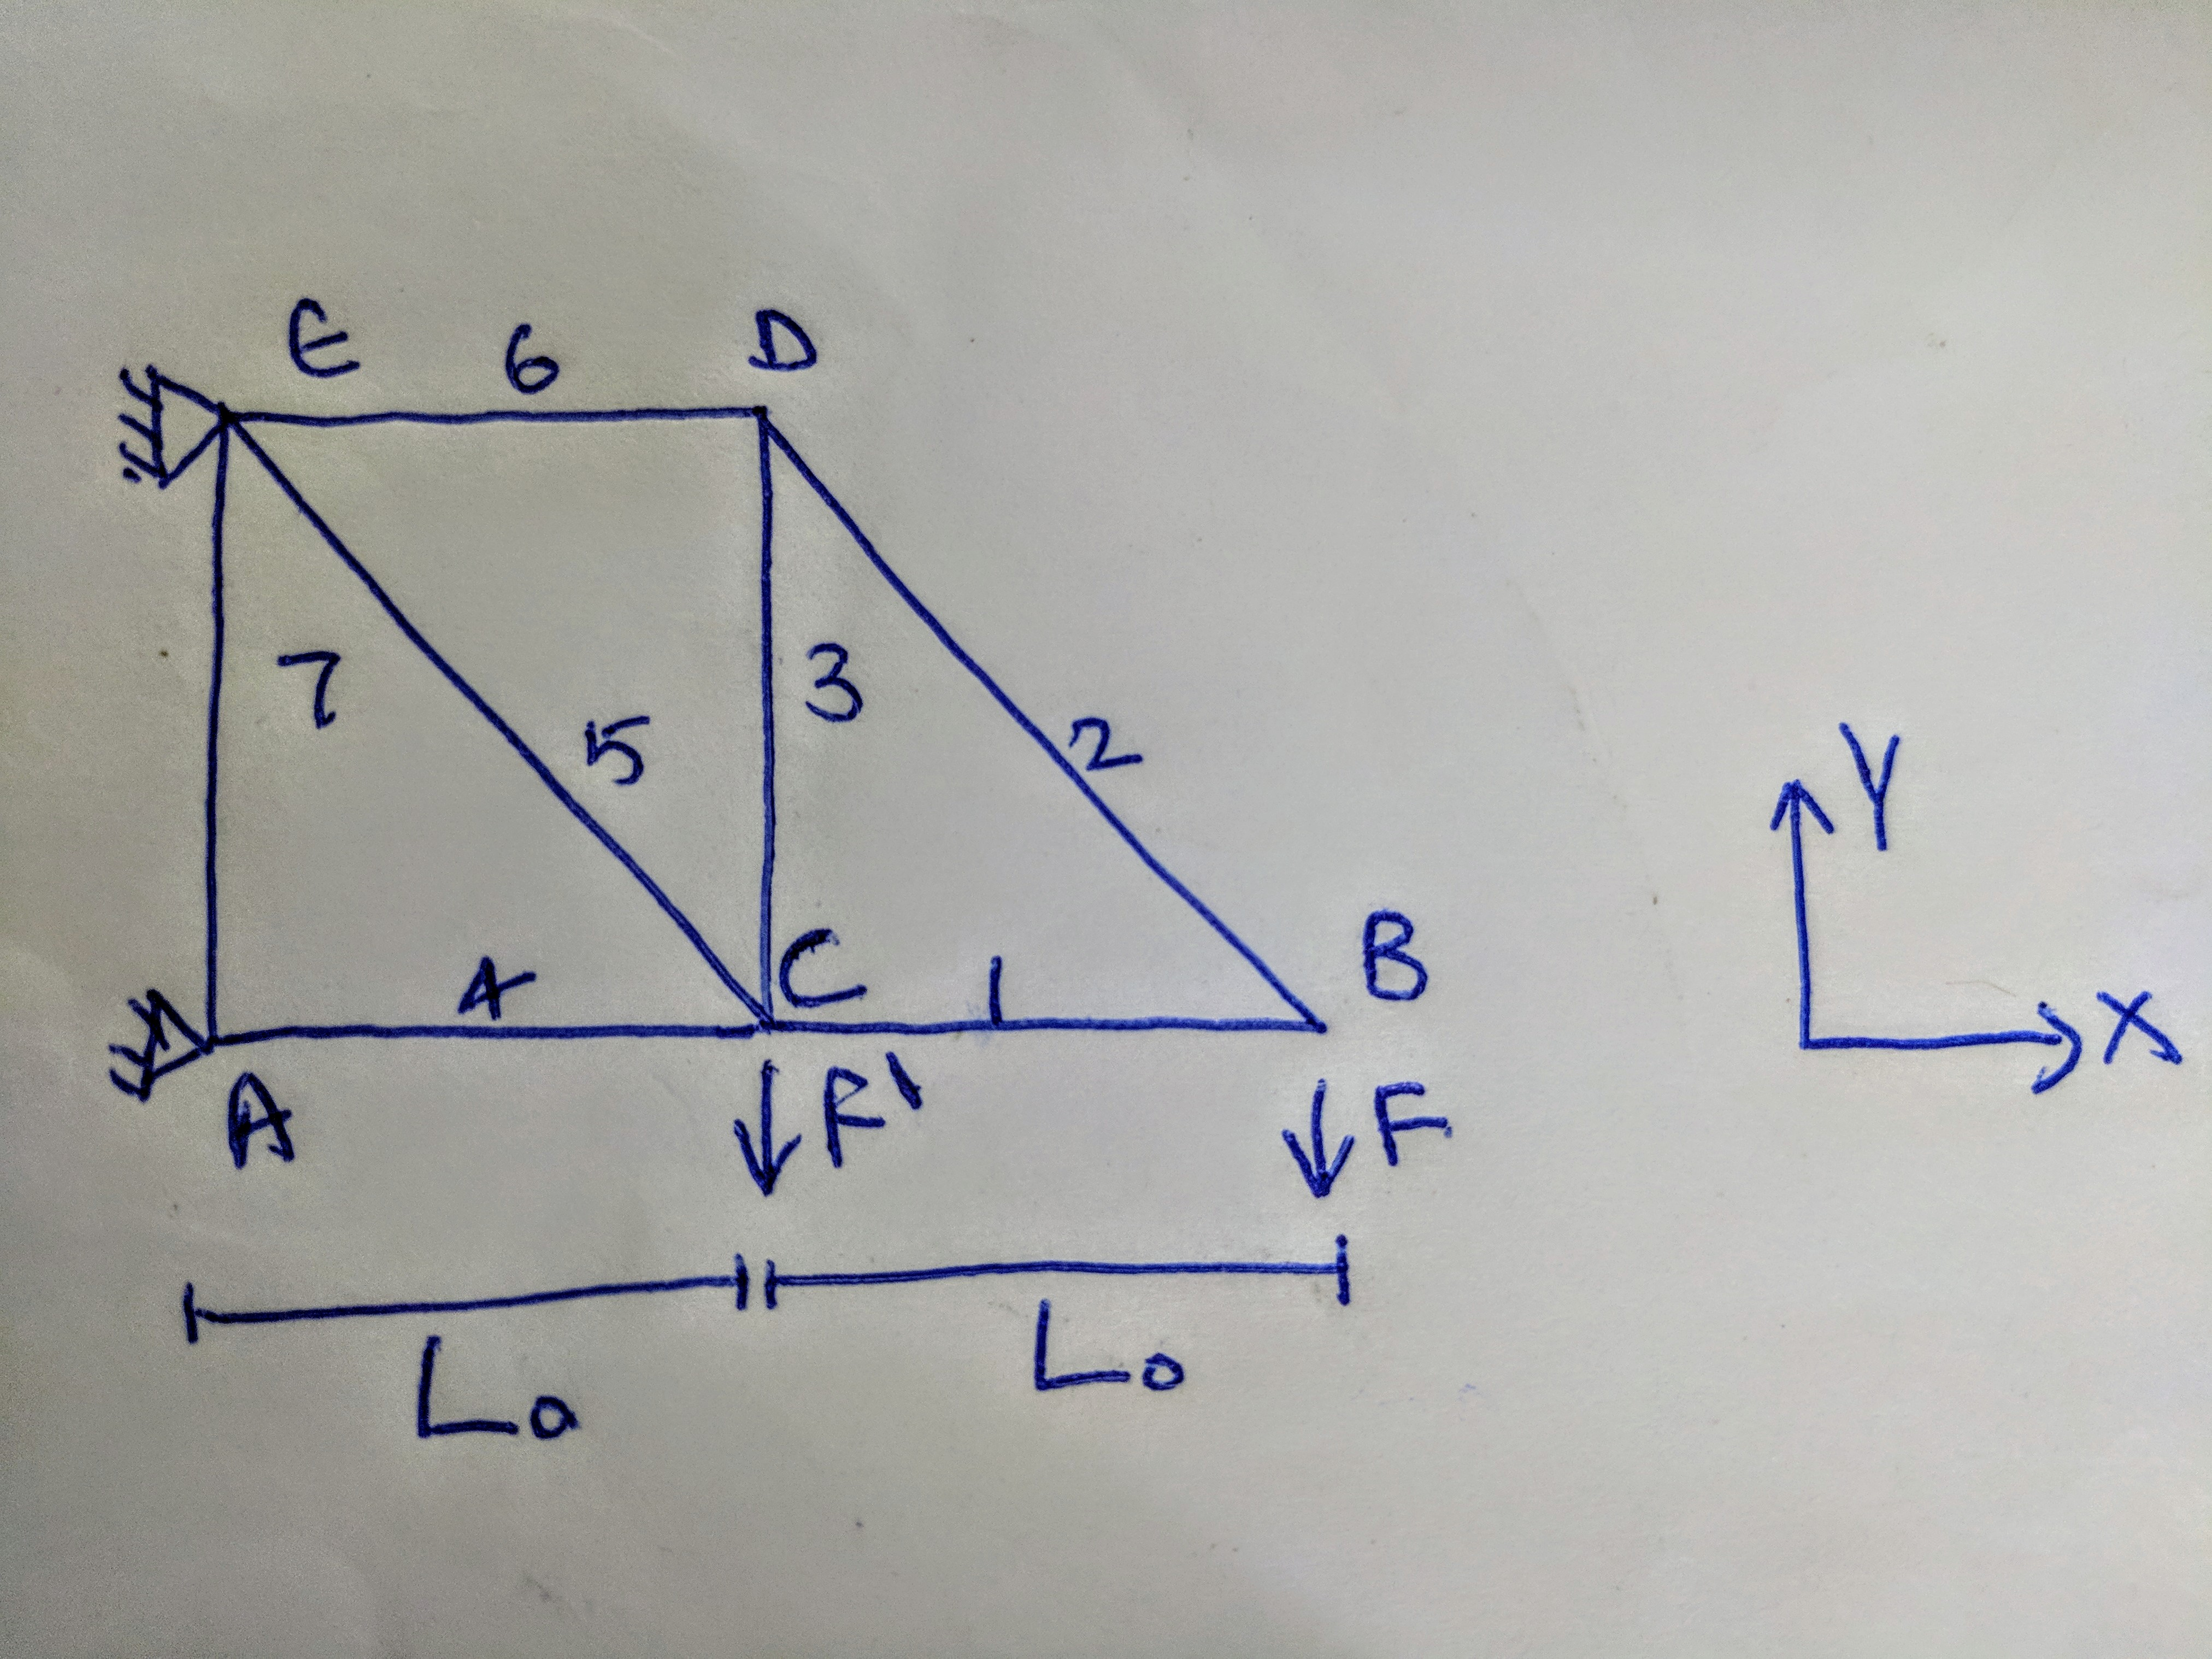
\includegraphics[scale=0.05]{Q2.jpg}

\noindent First, I will solve the structure to find the internal forces at each beam. Initially, I have assumed that the forces point towards the joint.\\
I am placing a fictitious force $F'$ at point C as we are required to find deflection at that point.\\
$P_i$ denotes force developed in beam $i$. \\

\noindent Force equilibrium equation for the overall system is $y$ direction:\\ 
$R_{VA}-R_{VD}-F-F'=0$\\
$\implies R_{VA}=R_{VD}+F+F'$\\

\noindent At point B:\\
Along $y: -F-\dfrac{P_2}{\sqrt{2}}=0$\\
$\implies P_2= -F\sqrt{2}$\\
Along $x: P_1+\dfrac{P_2}{\sqrt{2}}=0$\\
$\implies P_1=F$\\

\noindent At point D:\\
Along $y: P_3+\dfrac{P_2}{\sqrt{2}}=0$\\
$\implies P_3=F$\\
Along $x: P_6-\dfrac{P_2}{\sqrt{2}}=0$\\
$\implies P_6= -F$\\


\noindent At point C:\\
Along $y: -P_3-\dfrac{P_5}{\sqrt{2}}-F'=0$\\
$\implies P_5=-\sqrt{2}(F+F')$\\
Along $x: P_4+\dfrac{P_5}{\sqrt{2}}-P_1=0$\\
$\implies P_4=2F+F'$\\

\noindent At point A:
Along $y: -P_7+R_{VA}=0$\\
$\implies R_{VA}=P_7$\\

\noindent At point E:
Along $y: P_7+\dfrac{R_5}{\sqrt{2}}-R_{VD}=0$\\
$\implies P_7=0$\\

\noindent Energy $U=\sum\limits_{i=1}^7 \dfrac{P_i^2L_i}{2EA}$\\
$\implies U=\dfrac{1}{2EA}(P_1^2L_0+P_2^2L_0+P_3^2L_0+P_4^2L_0+P_5^2L_0\sqrt{2}+P_6^2L_0+P_7^2L_0)$ \\

\noindent $\implies U=\dfrac{L_0}{2EA}((9+2\sqrt{2})F^2+ (1+2\sqrt{2})F'^2 +(4+4\sqrt{2})FF')$\\

\noindent According to Castigliano's 2nd theorem, deflection at the beam at point C :\\
$\nu_C= \dfrac{\partial U}{\partial P'}\bigg \rvert_{F'=0}$\\
$\implies \nu_C=\dfrac{L_0}{2EA}(2(1+2\sqrt{2})F'+(4+4\sqrt{2})F)\Big \rvert_{F'=0}$\\

\noindent $\implies \mathbf{\nu_c=\dfrac{L_0}{EA}(2+2\sqrt{2})F}$\\

\bigbreak

\section{Question 3}

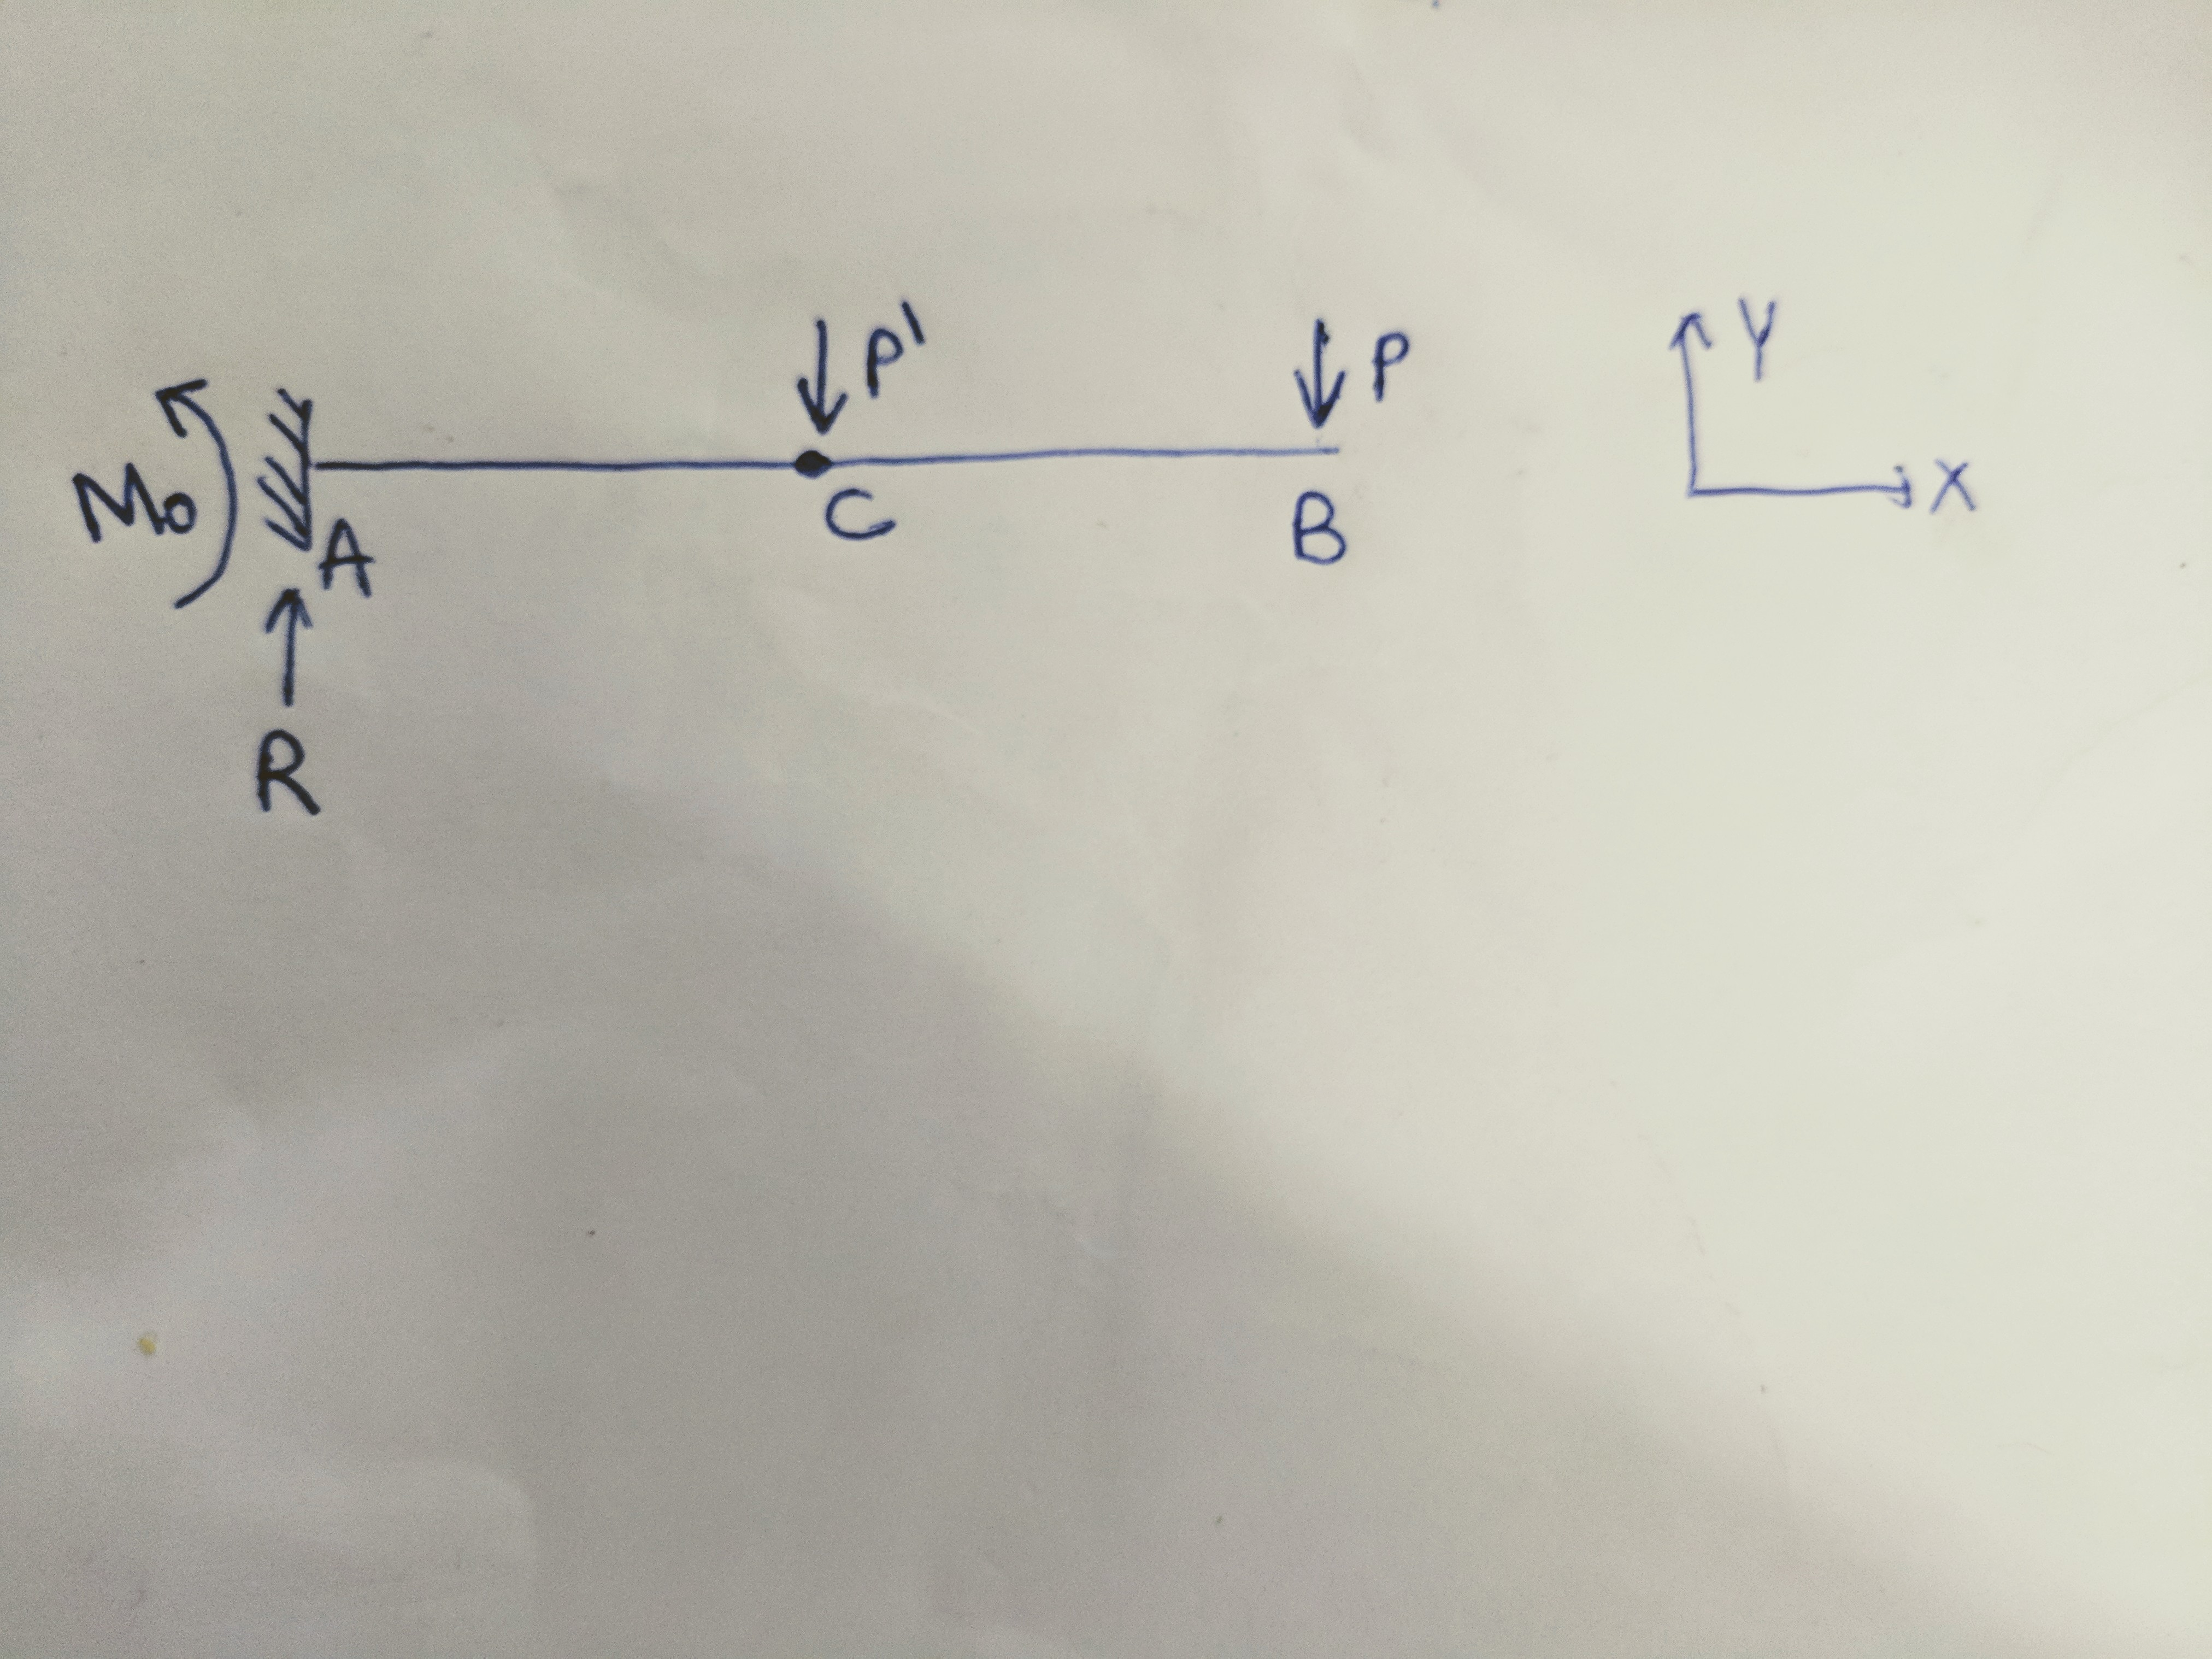
\includegraphics[scale=0.05]{Q3.jpg}

\noindent First we will solve the beam to determine reaction force and moment at the clamp. I am placing a fictitious force $P'$ at point $x=\dfrac{L}{2}$ as we are required to find deflection at that point.\\

\noindent Applying force equilibrium along $y$: \\
$R+P'-P=0$\\
$\implies R=P-P'$\\

\noindent Applying moment equilibrium about clamp:\\
$M_0-PL+\dfrac{P'L}{2}=0$\\
$\implies M_0=PL-\dfrac{P'L}{2}$\\

\noindent As $U=\bigint\limits_0^L\dfrac{M(x)^2}{2EI}dx$\\

\noindent Obtaining expression for $M(x)$:\\

\noindent For the region $0<x<\dfrac{L}{2}$:\\
Moment equilibrium about point X:\\
$\implies M_0-Rx+M=0$\\
$\implies M=P(x-L)-P'(x-\dfrac{L}{2})$\\

\noindent For the region $\dfrac{L}{2}<x<L$:\\
Moment equilibrium about point X:\\
$\implies M_0-Rx-P'(x-\dfrac{L}{2})+M=0$\\
$\implies M=Px-PL$\\

\noindent Now $U=\bigint\limits_0^L\dfrac{M(x)^2}{2EI}dx$\\
$\implies U=\bigint\limits_0^{L/2}\dfrac{(P(x-L)-P'(x-L/2))^2}{2EI}dx+\bigint\limits_{L/2}^L\dfrac{(Px-PL)^2}{2EI}dx$\\
$\implies U= \dfrac{1}{(P-P')}\bigg [\dfrac{7L^3P^3}{48EI}-\dfrac{L^3P'^3}{48EI} -\dfrac{L^3P^2P'}{4EI}+\dfrac{L^3PP'^2}{8EI} \bigg ] +\dfrac{L^3P^2}{48EI}$\\

\noindent According to Castigliano's 2nd theorem, deflection at the beam at $x=\dfrac{L}{2}$:\\
$\nu_{L/2}= \dfrac{\partial U}{\partial P'}\bigg \rvert_{P'=0}$\\
$\implies \nu_{L/2} = \dfrac{1}{(P-P')^2}\bigg [\dfrac{7L^3P^3}{48EI}-\dfrac{L^3P'^3}{48EI} -\dfrac{L^3P^2P'}{4EI}+\dfrac{L^3PP'^2}{8EI} \bigg ] +\dfrac{1}{(P-P')}\bigg [-\dfrac{L^3P'^2}{16EI} -\dfrac{L^3P^2}{4EI}+\dfrac{L^3PP'}{4EI} \bigg ] $\\
Substituting $P'=0$:\\
$\nu_{L/2}= \bigg [\dfrac{7L^3P}{48EI}\bigg ] +\bigg [ -\dfrac{L^3P}{4EI} \bigg ]$\\

\noindent $\implies \mathbf{\nu_{L/2}=-\dfrac{5L^3P}{48EI}}$\\

\noindent Negative sign indicates that deflection is in negative $y$ direction.
\end{document}
